\documentclass[10pt, a4paper]{article}

%\usepackage[utf8]{inputenc}

\usepackage{amsmath}
\usepackage{amsfonts}
\usepackage{amssymb}

\bibliographystyle{acm}
\usepackage{graphicx} 
\usepackage{rotating}

\usepackage{multicol}
\usepackage{url}

%\setcounter{secnumdepth}{0}

\usepackage{indentfirst} 
\setlength{\parindent}{5mm}

%\setlength{\marginparwidth}{1cm}
\usepackage[a4paper, top=30mm, bottom=30mm, left=25mm, right=25mm]{geometry}

\usepackage{titlesec} % Allows creating custom \section's\usepackage{url}
\titleformat{\section}
 {\normalfont\bfseries\large}{\arabic{section}    }{0em}{} % Section formatting
\renewcommand*{\thesection}{\arabic{section}}
\setlength\columnsep{7mm}

\begin{document}

\begin{center}
\Large
\textbf{Visualising Daily Solar Supply } \\ 
\hfill\\
\large
Joshua Maloney \\
School of Information Technology and Electrical Engineering \\
The University of Queensland, Qld., 4072, Australia \\
\hfill\\
\hfill\\
\end{center}


\begin{multicols}{2}

% Abstract
\begin{abstract}
%\textit{
%   Daily Solar supply is important.
%   Providing data on daily solar supply is novel.
%   The data is provided with a 3D interface.
%   Search through geographical areas.
%   View the data by visualising in natural ways.
%  }
\textit{
	SolarSupplyAu is a system for estimating and visualising the supply from photovoltaic sources each day in Australia. The system builds on existing provisions of data on current and future photovoltaic installations, geographic areas and daily weather. By combining this data, SolarSupplyAu provides an estimate of the energy provided from solar each day, which was not already readily available. SolarSupplyAu also uses 3D rendering techniques to show a visualisation of any suburb in Australia with its calculated daily supply and percentage of photovoltaic system coverage.	
}
\end{abstract}

\section{Introduction}

Solar supply is important because of goals 2020. We can see that the uptake of solar supply is at its highest rate ever. The amount of spending in solar is significant. 

Solar supply is provided by photovoltaic (PV) systems. In sunlight, PV systems provide electrical power which is measured in kilowatts (kW). Each day, we can say that a PV system provides an amount of solar energy, which is measured in kilowatt-hours (kWh).

We want to better understand some of this data, which is why we will capture it in a visualisation format. To really understand what to visualise, we have to look at the source data. 

The Australian Photovoltaic Institute (APVI)\cite{apvi} provides a key data set for this project. They have developed PVMap\cite{pvmap} which shows data on current and future installations. Note: the data comes from certified installations, however the actual pv system may be installed within 12 months of certification.

This dataset provides postcode data, which means we will also have to provide some mapping capabilities. 

Now that we know the installation size and where it is, we want to find out the daily weather data. The Bureau of Meteorology (BoM) gives daily gridded data sets on solar irradiance and temperature. 

With all this data, we hoped to show some useful information but it was not possible to find a way to calculate solar energy from this. 

We can look at how PV systems are producing power in real time using the online tool PVOutput\cite{pvoutput}. By studying this data, we can cross reference PV systems daily output with the weather files and produce a model for forecasting the output of other systems. We compute and provide this data which was not otherwise readily available. 

This finally gives us the ability to put a number on the solar energy supply of each postcode area, and sum to total for each state as well as the whole of Australia.

\section{Visualisation Design}

The visualisation is to show the data in a meaninful way, that helps the user find and understand what they are looking for. One of the key design factors is to be user friendly with an easy to use interface. 

Because we are dealing with suburb locations through a very large area, it was important to have ways to search. Findind data on a postcode area should be as simple as typing into a search box.

We used suburb names and postcodes from the ABS. There is a many-to-one association between locality names and postcode areas.

The terrain model is built from OpenStreetMap.

The building models come on top of that. 

The overall display begins at the country level. Initially we can choose to see the state breakdown, or go straight into search.  If we choose the state breakdown, we see each state and territory with its daily supply. At any time the search bar allows a zoomed in view of a single PCA, showing the landscape model and building model with percentage of pv installation, as well as figures for the daily supply for that postcode. 



\subsection{coding the visualisation}


\subsection{bringing the visualisation online}


\section{Node Design}

The Node collects daily data, performs the necessary calculations and formatting, finally providing the files that will be input to the visualisation. By doing this every day, the Node ensures that the visualisation will be showing current data.

\subsection{data collection}
\subsection{data processing}
\subsection{data delivery}
\subsection{automating the package (how to run everyday)}



%\subsection{Broad}
%
%This project describes the design and implementation of OpenSolar, including building the product system, the theory behind it's estimates and ways that it can be used. 
%
%The main part of OpenSolar is a visualisation that displays a 3D visualisation of photovoltaic (PV) sytems for any postcode region in Australia. The other major part of OpenSolar is a data processing backend that formats existing data and also estimates the daily power output.
%
%These values make it easy to find data on daily PV output. We provide data on PV sytem installations per residence, total capacity and daily power output for regions as small as a postcode area, and also display state and national totals.
%
%\subsection{Specific}
%
%The visualisation is made in WebGL and WebAssembly, because these technologies are available on all modern devices. Anyone can access the data and visualisation by using a web browser. 
%
%The data processing is calculated daily, using a docker container with a timed script to execute the process. 
%
%The two parts need to communicate, so that the daily data can be accessed by the visualisation. We host the visualisation on Github Pages, which loads a static page from a git repository. We give the docker container access to the same git repository, where it uploads the formatted data files.

%OpenSolar is designed to show daily solar supply with 3D visualisation. The data is sourced from APVI, BOM, ABS, OSM, OSMBuildings. The data to be visualised consists of solar energy produced by all systems calculated and updated daily, as well as regional coverage of small PV installations.

%The visualisation is constructed with OpenGL ES and c++. A compiler chain is used that outputs to a WASM binary. A website can load the application.

%To obtain the data, we use an offline process to calculate the source each day, and provide the processed data files directly to the site.

%The formula was developed with obesrvations from PVOutput and BOM.

%Data for solar supply can be calcluated for each postcode region, and is also grouped by state and a total supply is calculated for all regions in Australia. Before this tool, it was not possible to easily find the amount of solar energy generated daily. Now this data is available and can easily be explored by the accompanying visualisation.

%Zooming into the visualisation shows a 3D representation of the local area with buildings and elevation maps. 

% \message{The column width is: \the\columnwidth}
%The column width is: \the\columnwidth

% What is it
%Visualising Daily Solar Supply has produced the product OpenSolar. OpenSolar is a data processing and visualisation system. There are a number of dedicated applications as part of the system.

% What does it do
%OpenSolar gathers daily data and calculates the PV power generated in the previous day.

%OpenSolar can visualise solar power on a national scale, as well as zoom in to smaller, more focused geographic areas.

% Why is it so good
%How much solar power is generated per day nationally? This question is hard to answer and before OpenSolar, there was no estimate of such a value to be found.

%OpenSolar answers the question of how much power is being generated daily, as well as provides estimates on state, territory and postcode level.

%OpenSolar increases the understandability of the data by presenting it in a visually familiar way, using 3D maps to display recognisable locations.

%OpenSolar increasses ease of access to data by making the system available to users by a web browser, which is standard for modern devices including computers, tablets and phones.

%OpenSolar uses existing data services to make its calculations. This leverages existing sources to create new information.

%\includegraphics[scale=0.17]{design1.eps}

\section{Background}

% Why Solar?
Solar growing, millions of \$s, mandated energy targets.
Interest of PV to power companies.
Interest of PV to small system owners and community at large.

% What about 3D Visualisation?
3D visualisation is an easily available and accessible way to express solar supply. The data can be very dense, so 3D visualisation makes it more interesting.

% So how did you get to visualising it in a browser?
The solution is available on any device.

% What source data did you know you needed?
Some source data was provided. Some was missing. Part of the project was to find out what the missing data was.

% What source data did you find out you also needed?
We ended up asking how much solar power is generated each day? There wasn't a good answer, so to find out we had to dig up more data.

% Making preperation to develop the secret formula
By monitoring instantaneos output and daily solar irradaince we could come up with a relation between the current installed capacity and the daily solar power generation.

% Coding process for the visualisation
With all the background data together, the visualisation has everything needed to build a solid foundation.

Digital environment - emcc compiler, opengl, webcore. With this we can generate a blank canvas that we can work from.

Navigation

Postcode to lat-lon to 3d co-ordinate system.

UI

User interface to search for place or postcode.

High-Level viewing

Simple 3D map

Adding terrain - 3D geometry. 
Construct mesh grids. 
Adjust height and tile them together. 
Download and parse elevation tilesets from OSM. 
Mesh grids are uv mapped, which lets us show image tiles.

Adding buildings - 3D geometry

Representing the data in the geometry


% Container process for the estimation

% Centralising by Github

\section{Project Design}

% Kind of building and elaborating on the background

%\subsection{Explain the parts of the project}

%\subsection{Explain limitations of why it was caused to be that way}

\section{Results}

%\includegraphics[scale=0.17]{design1.eps}

\section{Conclusion}

Using this visualisation we can show PV coverage rates and pinpoint individual systems and their immediate output. We can show the projected daily output for postcode regions, and collect the data into state and country sized regions. We can display data that is generated daily using the previous day's latest solar data. 

We explore how the concept of a "virtual twin" city could use virtual space to integrate a number of data services.

We explore how the tool could be used to display relevant solar data.


\section*{Acknowledgement}

\section*{References}

\bibliography{bib_seminar}

\end{multicols}

\end{document}